\documentclass{article}
\usepackage[T2A]{fontenc}
\usepackage[utf8]{inputenc}
\usepackage[russian]{babel}
\usepackage{graphicx}

\begin{document}
\title{Рассмотрение зависимостей успеваемости студентов для разработки программы прогнозирующей успеваемость программы}
\author{Шупинский Владислав Александрович}
\date{\today}
\maketitle

\abstract{В статье рассматриваются демографические и социопсихологические факторы, а также методологии, на основе которых предсказывали успеваемость студентов.}

Для создания прогнозной модели успеваемости следует обратить внимание на факторы, на основе которых будет выстраиваться прогноз и методологии прогнозирования, а для этого стоит изучить уже имеющиеся научные статьи по тематике.
\section*{Зависимости успеваемости от различных факторов}
Рассматривая научные статьи для создания какого-либо прогноза, начинать стоит с рассмотрения зависимости, по этой причине первой рассмотрим \textit{«О некоторых зависимостях успеваемости студентов»} авторства Ерофина Е.А. и Хруслова Д.В. В этой статье авторами была рассмотрена успеваемость нескольких групп направлений связанных с IT технологиями. Выводы статьи говорят о том, что успеваемость напрямую зависит от понимания своей деятельности группой, хорошего расписания и наличия свободного времени. Стоит пояснить, что под \textit{«пониманием»} имеется в виду, что у групп, у которых практические и лабораторные опережали лекции средний балл был ниже, также те темы, что были перед зачетами, когда у студентов было мало времени были усвоены куда хуже остальных.[1]
Разумеется, следует также рассмотреть статью, посвящённую психологическим фактором, влияющим на успеваемость, для этого обратим внимание на статью \textit{«Взаимосвязь самооценки состояния здоровья и уровня заболеваемости с академической успеваемостью у студентов старших курсов медицинских специальностей с учетом влияния социально-экономических и демографических характеристик»} авторства Кузнецов В.В., Байрамов Р.А., Смирнов Е.А., Косилова Е.К., Косилов К.В. В статье описан эксперимент, по которому ясно видно, что чем выше процент людей с адекватной самооценкой по тесту Будасси, тем выше средний балл по группе. Обобщая выводы этой статьи, можно сказать, что чем удобнее расписание человека подогнано под его ритм жизни, тем эффективнее он сможет работать и успешнее будет [2]
\section*{Различные реализованные прогнозы}
Под конец следует рассмотреть статьи про само прогнозирование успеваемости. В статье \textit{«Анализ и прогнозирование успеваемости обучающихся при помощи использование цифровой образовательной среды»} авторства Шухмана А.Е., Парфенова Д.И., Легашева Л.В и Гришиной Л.С. обозревается не только само прогнозирование, но также и рассмотрены последствия перехода на дистанционное обучение. Студенты в целом показали не сильно более низкие результаты в связи с переходом на дистанционное обучение, но процент сдающих вовремя заметно снизился. Что касается прогнозирования, то прогноз успеваемости обучающихся опирается на внешние факторы: возраст, пол, состояние здоровья, результаты вступительных экзаменов, внеучебная деятельность студентов, в том числе временная или постоянная работы, участие в спортивных и общественно-культурных мероприятиях, а методология опирается на автоматизированную систему машинного обучения AutoML. [3] Среднее отклонение получилось примерно равным 0.2. Также рассмотрим статью \textit{«Прогнозирование успеваемости студентов на основе методов кластерного анализа»} авторства Шевченко В.А. В этой статье были рассмотрены несколько методов, и был выбран метод k-средних Мак-Кина, модифицированный под нужды задачи прогнозирования успеваемости. Формула - 
\[
    d_{ij} = \frac{1}{m} \sqrt{\sum_{k=1}^{m} ( z_ik - z_jk )^2}
\]  
Результат отличается от реальных оценок не более, чем на 3.3 процента, из чего в статье делается вывод о состоятельности метода.[4] 
\begin{figure}[h]
    \center{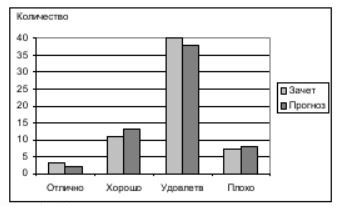
\includegraphics[scale=0.5]{TeX_ris_1.jpg}}
    \caption{Рис 1. Сравнительная таблица}
\end{figure}
\begin{tabular}{ | l | l | l | l | l | l | }
    \hline
      & Отлично & Хорошо & Удовлетворительно & Неудовлетворительно & Итого \\ \hline
    Зачетный балл & 3 & 11 & 40 & 7 & 61 \\
    Прогнозный балл & 2 & 13 & 38 & 8 & 61  \\
    \hline
\end{tabular}
И ещё в статье \textit{«Прогнозная модель для оценки успеваемости студентов университета по итогам текущего обучения»} авторства Зяблецева Павла Андреевича описана возможная модель прогнозирования успеваемости.
Также рассмотрим несколько англоязычных статей. \textit{«Predicting Academic Outcomes: A Survey from 2007 Till 2018»} авторства Sarah Alturki, Ioana Hulpuș, Heiner Stuckenschmidt рассматривает несколько нетипичную проблему, предсказывания потребности в литературе, основываясь на темах, по которым студенты получили низкие отметки. [6] Статья \textit{«Study on Student Performance Estimation, Student Progress Analysis, and Student Potential Prediction based on Data Mining»} авторства Michael Mogessie, Marco Ronchetti, Giuseppe Riccardi обозревает интеллектуальное решение, которое основываясь на оценках, а также личной информации о занятиях студентов в не учебное время определяет мешающие учебе факторы. [7] В статьях \textit{«Early Prediction of Student Learning Performance Through Data Mining: A Systematic Review»} авторства Javier López-Zambrano , Juan Alfonso Lara Torralbo , and Cristóbal Romero и \textit{«Predicting Student Performance Using Data Mining Techniques»} авторства A. Soni, Vivek Kumar, D. Hemavathi обозреваются применяемые методы предсказания успеваемости и делается вывод, что наиболее часто применяется линейная и логическая регрессии. [8,9] А в статье \textit{«COVID-19 and education: The lingering effects of unfinished learning»} авторства Emma Dorn, Bryan Hancock, Jimmy Sarakatsannis, and Ellen Virulego обозревается как пандемия сказалась на обучении. [10]
Рассмотрев все перечисленные статьи, можно сделать вывод, что предсказать оценки студента можно без учета текущих оценок и для этого лучше всего подойдёт кластеризация.
\section*{Библиографический список}
\begin{itemize}
    \item Ерофина Е.А. и Хруслова Д.В (2018). О некоторых зависимостях успеваемости студентов;
    \item Кузнецов В.В., Байрамов Р.А., Смирнов Е.А., Косилова Е.К., Косилов К.В. (2019). Взаимосвязь самооценки состояния здоровья и уровня заболеваемости с академической успеваемостью у студентов старших курсов медицинских специальностей с учетом влияния социально-экономических и демографических характеристик ;
    \item Шухман А.Е., Парфенов Д.И., Легашев Л.В., Гришина Л.С (2021). Анализ и прогнозирование успеваемости обучающихся при использовании цифровой образовательной среды: https://cyberleninka.ru/article/n/analiz-i-prognozirovanie-uspevaemosti-obuchayuschihsya-pri-ispolzovanii-tsifrovoy-obrazovatelnoy-sredy/viewer ;
    \item Шевченко В.А. (2015). Прогнозирование успеваемости студентов на основе методов кластерного анализа: https://cyberleninka.ru/article/n/prognozirovanie-uspevaemosti-studentov-na-osnove-metodov-klasternogo-analiza ;
    \item Зяблецев Павел Андреевич (2020). Прогнозная модель для оценки успеваемости студентов университета по итогам текущего обучения: http://earchive.tpu.ru/handle/11683/61074 ;
    \item Sarah Alturki, Ioana Hulpuș, Heiner Stuckenschmidt (2020). Predicting Academic Outcomes: A Survey from 2007 Till 2018: https://link.springer.com/article/10.1007/s10758-020-09476-0 ;
    \item Michael Mogessie, Marco Ronchetti, Giuseppe Riccardi (2017). Study on Student Performance Estimation, Student Progress Analysis, and Student Potential Prediction based on Data Mining ;
    \item Javier López-Zambrano , Juan Alfonso Lara Torralbo , and Cristóbal Romero (2018). Early Prediction of Student Learning Performance Through Data Mining: A Systematic Review;
    \item A. Soni, Vivek Kumar, D. Hemavathi (2018). Predicting Student Performance Using Data Mining Techniques ;
    \item Emma Dorn, Bryan Hancock, Jimmy Sarakatsannis, Ellen Virulego (2021). COVID-19 and education: The lingering effects of unfinished learning: https://www.mckinsey.com/industries/education/our-insights/covid-19-and-education-the-lingering-effects-of-unfinished-learning .
\end{itemize}
\end{document}  